\documentclass{article}
\usepackage{bookmark}
\usepackage{color}
\usepackage{amsmath}
\usepackage{hyperref}
\usepackage{listings}
\usepackage{xcolor}
\usepackage{indentfirst}
\usepackage{graphicx}
\usepackage{amsfonts}
\usepackage{hyperref}
\usepackage[top=2cm, bottom=2cm, left=2cm, right=2cm]{geometry}  
\usepackage{algorithm}  
\usepackage{algorithmicx}  
\usepackage{algpseudocode} 
 
\renewcommand{\algorithmicrequire}{\textbf{Input:}}  
\renewcommand{\algorithmicensure}{\textbf{Output:}}  

\begin{document}
{\noindent {\bf Ex 1.} 1. (a) First is to prove that there exists a number $x_0$ such that for $x>x_0$, $x^3-3x^2-x+1\geq cx^3$, which means that $\frac{x^3}{x^3-3x^2-x+1}\leq \frac{1}{c}$.

Because $\lim\limits_{x\rightarrow\infty}\frac{x^3}{x^3-3x^2-x+1}=1$, which means that for any number $\delta>0$, there exists a number $\epsilon$ that $\frac{x^3}{x^3-3x^2-x+1}<1+\delta$ when $x>\epsilon$

Let $c = \frac{1}{1+\delta}, x_0=\epsilon$, it can be easily seen that $n^3-3n^2-n+1=\Omega (n^3)$

And $n^3-3n^2-n+1=O(n^3)$ can be proved in the similar way. So it can be concluded that $n^3-3n^2-n+1=\Theta (n^3)$\\

{\noindent (b) It is to prove that there exists a number $x_0$ such that for $x>x_0$, $x^2\leq c2^x$, which is to say that $\frac{x^2}{2^x}<c$.}

Extract the logarithm, the inequality will be $2lnx-xln2<lnc$, which is $\frac{2lnx-lnc}{x}<ln2$

Because $\lim\limits_{x\rightarrow\infty}\frac{2lnx-lnc}{x}=0$, it is obvious that such $x_0$ exists, so $n^2=O(2^n)$\\

{\noindent 2. (a) $n\sqrt{n} = O(n^2-1)$\\}

{\noindent 3. (a) There is no such pair. (b) $f(n)=n^2-1,g(n)=n\sqrt{n}$\\}

{\noindent 4. $f_2,f_3,f_1,f_4$\\}
\hrule

\vskip 2em

{\noindent {\bf Ex 2.} 1. (a) The recursion tree is shown below.}

\begin{figure}[h]
    \centering
    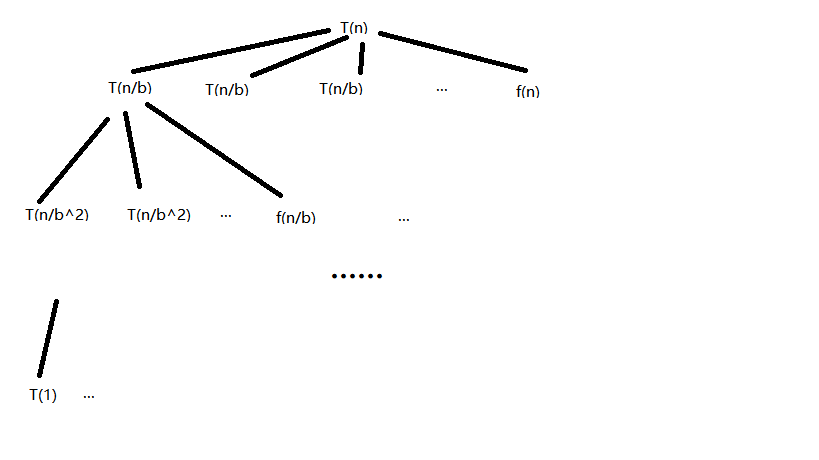
\includegraphics[scale=0.5]{1.png}
\end{figure}

{\noindent (b) i. The depth is $log_bn+1$\\}

{\noindent ii. Number of leaves is $\sum_{k=0}^{log_bn}a^k = \frac{a^{log_bn+1}-1}{a-1}$\\}

{\noindent iii. Suppose the depth of the root is 0, then the cost on the $k_{th}$ depth is $$a^{k-1}f(\frac{n}{b^{k-1}})$$ for $0<k<log_bn$, $0$ for $k=0$ and $a^{log_bn-1}f(b)+a^{log_bn}T(1)$ for $k=log_bn$\\

{\noindent iv. It can be seen that $$T(n)=\sum_{k=1}^{log_bn}a^{k-1}f(\frac{n}{b^{k-1}})+a^{log_bn}T(1) = \frac{T(1)}{a}n^{log_ba}+\sum_{j=0}^{log_bn-1}a^jf(\frac{n}{b^j})=\Theta(n^{log_ba})+\sum_{j=0}^{log_bn-1}a^jf(\frac{n}{b^j})$$}

{\noindent 2. (a). i. It can be seen that $c_1(\frac{n}{b^j})^{log_ba}\leq f(\frac{n}{b^j})\leq c_2(\frac{n}{b^j})^{log_ba}$ for $n>n_0$

So $c_1\sum_{j=0}^{log_ba-1}a^j(\frac{n}{b^j})\leq g(n)\leq c_2\sum_{j=0}^{log_ba-1}a^j(\frac{n}{b^j})$ when $n>n_0$, and consequently $g(n)=\Theta(\sum_{j=0}^{log_ba-1}a^j(\frac{n}{b^j})^{log_ba})$\\

{\noindent iii. Because actually $$\sum_{j=0}^{log_ba-1}a^j(\frac{n}{b^j})^{log_ba}=n^{log_ba}log_bn$$}

So $$g(n)=\Theta(n^{log_ba}log_bn)$$\\

{\noindent (b). ii. This is the partial sum of a geometric sequence starting from $n^{log_ba-\epsilon}$, with ratio $\frac{a}{b^{(log_ba-\epsilon)}}$ and $log_bn$ terms so it is $$n^{log_ba-\epsilon}\frac{\frac{a}{b^{(log_ba-\epsilon)}}^{log_bn}-1}{\frac{a}{b^{(log_ba-\epsilon)}}-1}=\frac{n^{\epsilon}-1}{b^{\epsilon}-1}n^{log_ba-\epsilon}$$}

{\noindent iii. From 1 and 2, it can be concluded that $g(n)=O(\frac{n^{\epsilon}-1}{b^{\epsilon}-1}n^{log_ba-\epsilon})=O(n^{log_ba})$}\\

{\noindent (c).i. It is obvious because $g(n)$ has a $f(n)$ term in it, and all terms are larger than or equal to $0$, so it is always larger than or equal to $f(n)$ }\\

{\noindent ii. $a^jf(\frac{n}{b^j})\leq a^{j-1}cf(\frac{n}{b^{j-1}})\leq ...\leq c^jf(n)$}\\

{\noindent iv. Because $g(n)$ is both $O(f(n))$ and $\Omega (f(n))$, so it is $\Theta (f(n))$\\

\hrule
\vskip 2em

{\noindent {\bf Ex 3. } The algorithm is shown below.}


\begin{algorithm}[H]  
    \caption{Ramanujam Number Finding}  
    \begin{algorithmic}[1]  
        \Require A number $n$
        \Ensure All Ramanujam numbers smaller than $n$
            \State $T \gets \{\}$
            \For {$i = 1 \to n$}
                \For {$j = 1 \to \lfloor \sqrt[3]{i} \rfloor$}
                    \If {$i-j^3 \text{ is a cubic number}$}
                        \For {$k = j+1 \to \sqrt[3]{i-j^3}-1$}
                            \If {$i-k^3 \text{ is a cubic number}$}
                                \State $T\gets T+\{i\}$
                            \EndIf
                        \EndFor
                    \EndIf
                \EndFor
            \EndFor
            \State \Return $T$
              
    \end{algorithmic}  
\end{algorithm}

The complexity is $O(n(\sqrt[3]{n})^2)$\\

\hrule 
\vskip 2em

{\noindent {\bf Ex 4. } Suppose only pirate 5 and 6 remains. Of course pirate 6 will not agree with pirate 5 until pirate 5 give all coins to pirate 6, so the distribution must be zero for pirate 5 and 300 for pirate 6.}

Then consider the situation when there are pirate 4, 5 and 6. Winning the vote from pirate 5 is very easy for pirate 4 because he only need to give pirate 5 one coin, which is larger than his profit if pirate 4 is dead. And he need not to care pirate 6 because he has won pirate 5's vote. So the distribution will be 299 for pirate 4, 1 for pirate 5 and 0 for pirate 6.

When there are pirate 3,4,5,6, what pirate 3 should do is to raise profit of pirate 6 to 1 and then give pirate 4 and 5 no coin. So the distribution will be 299 for pirate 3, 0 for pirate 4 and 5, 1 for pirate 6.  

When there are pirate 2,3,4,5,6, what pirate 2 should do is to raise profit of pirate 4 and 5 to 1 and then give pirate 3 and 6 no coin. So the distribution will be 298 for pirate 2, 0 for pirate 3 and 6, 1 for pirate 4 and 5. 

When there are pirate 1,2,3,4,5,6, what pirate 1 should do is to raise profit of pirate 3 and 6 to 1 and then give pirate 2,4 and 5 no coin. So the final distribution will be 298 for pirate 1, 0 for pirate 2,4 and 5, 1 for pirate 3 and 6. Pirate 1 will win the vote from pirate 3,6 and himself\\


\end{document}